% Provenance (never printed): see sources/outline_sources.md (Year 3: gravity, magnetic,
% seismic, resistivity and ground-penetrating-radar surveys; data processing and
% uncertainty; a mapping project).
% Brief: sources/book5/BRIEFS.md, ch. 31. Curves from figdata/bachelor-3/gravity_granite.py
% (prism model of the Varden granite of figdata/shared/region.py), magnetic_dyke.py (2-D
% dyke; the Varden dolerite dyke of the Sync 3 ruling, buried below the unconformity),
% resistivity_sounding.py (Pekeris transform and image series) and gpr_radargram.py.
% Physical-property ranges and survey practice from the GPG open textbook (CC BY 4.0) and
% Keys (1990). Exercise and problem values in the Book 5 scratch calculator calc/ch31.py.
\chapter{野外与实验室方法 III}\label{ch:b3:field-lab-methods-3}

一支地球物理勘探小组在瓦尔登丘陵的山谷中工作一周。瓦尔登丘陵是一个虚构的地区，
其地质图曾由本科一年级分册在地质图一章中绘出，
图上显示，一层花岗岩露头于山谷两侧，
夹在片岩之间，位于覆于两者之上的砂岩之下。
花岗岩在覆盖层之下延伸到何处、
延伸多远、深埋多深，无人见过。小组携带一台重力仪、两台磁力仪、
一条电极电缆和一台雷达，
都装在一辆小推车上。这些仪器没有一台能直接看到岩石：
每一台仪器测量的都是地表的一个场——重力、磁场、电势、
无线电脉冲的回波——而下方的岩石会扰动这些场。
一周结束时，小组能画出它从未见过的花岗岩，
说出谷底冲积层有多深，
并报告一个任何地图都未标出的磁性体。

本章循着这一周展开。各种方法依次讨论，
每种方法既是带改正的测量，
也是以若干几何体为对象的\omterm{def:b3:seismology-imaging:inverse}{正演问题}，这些几何体的场可以精确算出；
随后说明勘探误差如何累积，以及为何一类数据通常不足以确定模型；
最后以瓦尔登勘探收尾，
将各种方法综合在一起。

\begin{recall}
重力异常、自由空气校正与布格校正及其异常，
以及正常重力，均见于本科一年级分册中关于地壳均衡与重力的一章；
\omterm{def:b3:field-lab-methods-3:gravimeter}{相对重力仪}的测量环路见于
\cref{ch:b3:gravity-geodesy}。主磁场及其\omterm{def:b3:palaeomagnetism:inclination}{磁倾角}、
\omterm{thm:b3:palaeomagnetism:dipole}{偶极子公式}与\omterm{def:b3:palaeomagnetism:igrf}{国际地磁参考场}见于
\cref{ch:b3:palaeomagnetism}。电阻率、欧姆定律与相对
介电常数、电磁波、磁化强度与
磁化率见于物理学书籍，高斯定理（用于重力）
亦在其中。\omterm{def:b3:exploration-seismology:surveys}{地震折射勘探}见于
\cref{ch:b3:exploration-seismology}；\omterm{def:b3:seismology-imaging:inverse}{正演问题}、\omterm{def:b3:seismology-imaging:inverse}{反演问题}及
加权最小二乘见于\cref{ch:b3:seismology-imaging}；孔隙度见于
中学课本，\omterm{def:b3:facies-models:wireline}{测井曲线}见于\cref{ch:b3:facies-models}。
不确定度的传播见于化学书与数学书。
\end{recall}

\section{重力勘探}\label{sec:b3:field-lab-methods-3:gravity}

重力勘探所寻找的异常很小。赤道处的重力约为
\qty{978000}{\milli\gal}；大型构造可使其改变数百毫伽，盐丘约改变十毫伽，
矿体约改变一毫伽，工程地质勘探的目标仅改变
百分之几毫伽。地球物理学家以毫伽
为单位计量，有时也以\qty{0.1}{\milli\gal}为单位；一项有用的勘探
必须能分辨相对于
$g$ 的亿分之一的差异。
% ledger: gpg:grav-units, gpg:grav-sizes

\begin{definition}[相对重力仪；仪器漂移]\label{def:b3:field-lab-methods-3:gravimeter}
称\emph{相对重力仪}\index{相对重力仪}为一种测量各站间重力差的仪器：
其核心为一个挂在弹簧上的质量块，由第二个可调的力保持在零位，
其刻度读数乘以标定常数，即得以毫伽计的重力值，但差一未知常数。其\emph{仪器
漂移}\index{仪器漂移}是指同一固定测站上读数随时间的缓慢变化，
由弹簧蠕变、温度变化和震动引起；
其测定方法是：隔数小时后，
重读一个已读过的测站，
此测站即
\emph{基站}。
\end{definition}
% ledger: gpg:gravimeter, gpg:grav-survey

野外重力仪的量程为数万毫伽，
读数精度最佳约为\qty{0.01}{\milli\gal}；量程须在运输后重新设定。
在此精度下，每个测站的高度与读数同等重要：
\qty{3.3}{cm}的高度误差即足以损害\qty{0.01}{\milli\gal}的精度，
因此测站位置须用卫星接收机或精确到厘米的水准仪测定。
基站每隔约两小时重测一次。
固体地球潮汐的幅度可达
\qty{0.3}{\milli\gal}，在这几小时内变化足够缓慢，
可随漂移一并扣除。
% ledger: gpg:gravimeter, gpg:grav-survey, gpg:grav-sizes

\begin{method}[重力环路的化算]\label{met:b3:field-lab-methods-3:loop}
一个环路从基站出发并回到基站，两次读数的时刻分别为 $t_0$ 和 $t_1$。
\begin{enumerate}
  \item 由两次基站读数计算漂移速率 $(r_1 - r_0)/(t_1 - t_0)$；
        其中包含潮汐的影响。
  \item 从每次读数中减去自 $t_0$ 以来积累的漂移，
        即 $r - (t - t_0)(r_1 - r_0)/(t_1 - t_0)$，并减去基站
        读数，即得相对于基站的重力。
  \item 对测站高出基站的高度 $\Delta h$ 作改正：
        加上自由空气校正 $\qty{0.3086}{\milli\gal.m^{-1}}
        \times\Delta h$，并减去布格校正
        $\qty{0.1119}{\milli\gal.m^{-1}}\times\Delta h$（密度
        \qty{2670}{kg.m^{-3}}），即加上 $0.1967\,\Delta h$。
  \item 对位于基站以北距离 $\Delta y$ 处的测站，减去
        正常重力的变化，$\qty{0.811}{\milli\gal.km^{-1}}
        \times\sin 2\varphi\times\Delta y$。
  \item 加上各测站的\omterm{def:b3:field-lab-methods-3:terrain}{地形校正}。
\end{enumerate}
结果即相对于基站的布格异常。将基站与绝对重力已知的测站联测，
即可得到异常本身。
\end{method}
% ledger: gpg:grav-survey, gpg:terrain

布格校正把测站与参考面之间的地层当作平板。
实际地形中，这一处理在两方面都有误：
高出测站的山丘向上拉引，使读数偏低；
低于测站的山谷在平板中被算作
并不存在的岩石。

\begin{definition}[地形校正]\label{def:b3:field-lab-methods-3:terrain}
重力测站的\emph{地形校正}\index{地形校正}，
是地形偏离布格平板的部分对测站施加的引力：
测站水准面以上的山丘，以及
其下方的山谷，均按平板密度计入。两者都使
实测重力比平板值偏小，因此修正量
总是加上。
\end{definition}

过去借助哈默图与数表手工计算，逐区
由测站向外推进；如今改由数字高程模型计算。
远离陡峭地形时，它很少超过 \qty{1}{\milli\gal}，
但靠近测站的分区很难算准，
修正量很少能精确到优于 \qty{0.2}{\milli\gal}。
% ledger: gpg:terrain, gpg:grav-sizes

\subsection{简单形体的异常}

重力\omterm{def:b3:seismology-imaging:inverse}{正演问题}是一个求和：形体的每一微元（
密度差为 $\Delta\rho$）依牛顿定律吸引测站，
而测量的是该和的竖直分量。少数形体可
直接给出封闭形式的结果。

\begin{theorem}[球体与水平圆柱体]\label{thm:b3:field-lab-methods-3:sphere}
在距球心正上方水平距离为 $x$ 处，埋藏的
剩余质量为 $\Delta m$、球心位于深度 $z$ 的球体
给出异常：
\[
\Delta g(x) = \frac{G\,\Delta m\,z}{(x^2 + z^2)^{3/2}} ,
\]
异常降至峰值一半处的水平距离为 $x_{1/2} = z\sqrt{2^{2/3} - 1}$，
即 $z = 1.305\,x_{1/2}$。长水平圆柱体单位长度的剩余质量
为 $\lambda$，轴线位于深度 $z$，沿
垂直于其走向的剖面给出
\[
\Delta g(x) = \frac{2G\lambda z}{x^2 + z^2} ,
\]
且 $z = x_{1/2}$。
\end{theorem}

\begin{proof}
对于密度仅依赖于到球心距离的球体，其外部引力
等同于把其质量集中于球心所产生的引力（
壳定理，是高斯定理的推论）。测站处引力的大小
为 $G\Delta m/(x^2 + z^2)$，竖直分量带有
因子 $z/\sqrt{x^2 + z^2}$。令 $\Delta g(x_{1/2}) =
\Delta g(0)/2$，得 $(1 + x_{1/2}^2/z^2)^{3/2} = 2$，由此即得上述规则。对于
圆柱体，在半径为 $r$ 的同轴圆柱面上应用高斯定理，得
场为 $2G\lambda/r$，竖直分量为 $2G\lambda z/r^2$；
当 $x^2 + z^2 = 2z^2$ 时达到峰值的一半。
\end{proof}
% ledger: gpg:half-width

非球形形体同样有半宽，此时由该规则
得出的是等效球体的深度，而非形体本身的深度。该规则
只是一个初步估计，在拟合任何模型之前作出。

\begin{proposition}[轴线上的竖直圆柱体]\label{prop:b3:field-lab-methods-3:vcyl}
半径为 $a$、密度差为 $\Delta\rho$ 的竖直圆柱体，
其顶面与底面位于测站以下深度 $z_1 < z_2$ 处，
则其轴线上给出
\[
\Delta g = 2\pi G\Delta\rho\left[(z_2 - z_1) + \sqrt{z_1^2 + a^2}
           - \sqrt{z_2^2 + a^2}\right] .
\]
当 $a \to \infty$ 时即为布格平板 $2\pi G\Delta\rho(z_2 - z_1)$；
对于从地表延伸到很大深度的圆柱体，它趋于
$2\pi G\Delta\rho\,a$。
\end{proposition}

\begin{proof}
半径为 $a$、厚度为 $\mathrm{d}z$ 的圆盘，在深度 $z$ 处对其轴线上
一点的吸引为 $2\pi G\Delta\rho\,\mathrm{d}z\,(1 -
z/\sqrt{z^2 + a^2})$，即圆环的引力
对半径积分。从 $z_1$ 积到 $z_2$ 即得括号项。当 $a \to
\infty$ 且深度固定时，$\sqrt{z_1^2 + a^2} - \sqrt{z_2^2 + a^2} =
(z_1^2 - z_2^2)/(\sqrt{z_1^2 + a^2} + \sqrt{z_2^2 + a^2}) \to 0$；当
$z_1 = 0$ 且 $z_2 \to \infty$，$z_2 - \sqrt{z_2^2 + a^2} \to 0$ 且
括号项趋于 $a$。
\end{proof}

\begin{proposition}[由重力图求剩余质量]\label{prop:b3:field-lab-methods-3:gauss}
不论完全位于某水平面以下的形体具有何种形状，
其剩余质量为
\[
\Delta m = \frac{1}{2\pi G}\iint \Delta g\,\mathrm{d}A ,
\]
积分范围为整个水平面。
\end{proposition}

\begin{proof}
对于点质量 $m$，其深度为 $z$，$r$ 为水平距离，则
$\iint \Delta g\,\mathrm{d}A = \int_0^\infty
Gmz\,(r^2 + z^2)^{-3/2}\,2\pi r\,\mathrm{d}r = 2\pi Gm$：穿过平面的恰是
高斯定理中通量 $4\pi Gm$ 的一半。形体是点质量之和，
而积分是线性的。
\end{proof}

该定理只给出质量，不给出形状；而一幅图只覆盖平面的
一部分，且深埋形体的异常衰减缓慢，因此
由图求得的质量偏小，除非借助模型把其边缘
向外延拓。

\begin{omfigure}
\begin{tikzpicture}
\begin{axis}[axis equal image, xmin=1.5, xmax=5.5, ymin=2.6, ymax=5.7, width=0.86\linewidth,
  tick label style={font=\scriptsize}, xlabel={东 (km)}, ylabel={北 (km)},
  label style={font=\small}, unbounded coords=jump]
% geology of the region (figdata/shared/region.py), faded
\addplot[lith schist, draw=black!50, line width=0.2pt, even odd rule, opacity=0.45] table {figdata/out/shared-region-unit-schist.dat};
\addplot[lith granite, draw=black!50, line width=0.2pt, even odd rule, opacity=0.45] table {figdata/out/shared-region-unit-granite.dat};
\addplot[om lith={icsTriassic!35}{om sand}, draw=black!50, line width=0.2pt, even odd rule, opacity=0.45] table {figdata/out/shared-region-unit-sandstone.dat};
\addplot[om lith={icsJurassic!40}{om limestone}, draw=black!50, line width=0.2pt, even odd rule, opacity=0.45] table {figdata/out/shared-region-unit-limestone.dat};
\addplot[om lith={icsJurassic!15}{om shale}, draw=black!50, line width=0.2pt, even odd rule, opacity=0.45] table {figdata/out/shared-region-unit-shale.dat};
\addplot[lith alluvium, draw=black!50, line width=0.2pt, even odd rule, opacity=0.45] table {figdata/out/shared-region-unit-alluvium.dat};
\addplot[river] table {figdata/out/shared-region-river.dat};
% the survey (figdata/bachelor-3/gravity_granite.py, magnetic_dyke.py)
\addplot[only marks, mark=*, mark size=0.7pt, black!70] table[x=x_km, y=y_km] {figdata/out/bachelor-3-gravity_granite-stations.dat};
\addplot[omDef, very thick] table[x=x_km, y=y_km] {figdata/out/bachelor-3-gravity_granite-contours.dat};
\addplot[omThm, thick] coordinates {(1.5,4.15) (5.5,4.15)};
\addplot[omMeth, line width=2.2pt, opacity=0.8] coordinates {(1.7,4.15) (2.7,4.15)};
\addplot[omProp, dashed, thick] coordinates {(2.2,2.6) (2.2,5.7)};
\addplot[only marks, mark=star, mark size=3.5pt, omMeth!70!black, thick] coordinates {(3.5,4.0)};
\node[font=\scriptsize, fill=white, fill opacity=0.85, text opacity=1, inner sep=1pt] at (axis cs:3.5,5.12) {$-0.5$};
\node[font=\scriptsize, fill=white, fill opacity=0.85, text opacity=1, inner sep=1pt] at (axis cs:3.5,4.84) {$-1$};
\node[font=\scriptsize, fill=white, fill opacity=0.85, text opacity=1, inner sep=1pt] at (axis cs:3.5,4.58) {$-2$};
\node[font=\scriptsize, anchor=south west, fill=white, fill opacity=0.85, text opacity=1, inner sep=1pt] at (axis cs:1.55,4.17) {重力剖面};
\node[font=\scriptsize, anchor=north, fill=white, fill opacity=0.85, text opacity=1, inner sep=1pt] at (axis cs:2.2,4.08) {磁测线};
\node[font=\scriptsize, anchor=north west, text=omProp!80!black, fill=white, fill opacity=0.85, text opacity=1, inner sep=1pt] at (axis cs:2.24,5.6) {埋藏岩墙};
\node[font=\scriptsize, anchor=north, fill=white, fill opacity=0.85, text opacity=1, inner sep=1pt] at (axis cs:3.5,3.92) {测深点};
\pic at (axis cs:5.15,5.3) {northarrow};
\end{axis}
\end{tikzpicture}

\par\smallskip{\small 瓦尔登测区的测量结果叠加于该地区的地质图上
（底图褪色：片岩为灰色，花岗岩为粉色，覆盖层的
砂岩、石灰岩和页岩，以及沿河的冲积物）。黑点：重力测点，
相距 \qty{200}{m}；蓝色：花岗岩模型的布格异常，
等值线间距 \qty{0.5}{\milli\gal}；红色：重力剖面；绿色：
谷底的磁测线与电测深点（星号）；
橙色虚线：磁测发现的辉绿岩岩墙，
埋藏于覆盖层之下。}\label{fig:b3:field-lab-methods-3:survey}
\end{omfigure}
% ledger: gpg:densities

\subsection{瓦尔登花岗岩}

地质学家给出的花岗岩模型是一个椭球形岩体，位于
不整合面之下，东西向跨度 \qty{760}{m}，南北向跨度 \qty{1120}{m}
（与覆盖层相接处），岩体向下逐渐变宽；在
谷壁处延伸至地表。花岗岩比片岩轻：
已发表的密度范围为 \numrange{2.50}{2.81} 及
\qtyrange{2.39}{2.80}{g.cm^{-3}}。测量模型取
\qty{2620}{kg.m^{-3}} 作为花岗岩的密度，\qty{2750}{kg.m^{-3}} 作为
片岩的密度，两者密度差为 \qty{-130}{kg.m^{-3}}，并将花岗岩底面止于
海平面以下 \qty{1500}{m} 处，这是一个假设，因为没有任何资料显示其
底面位置。将模型剖分为 \num{5533} 个直棱柱体，其引力
具有闭合形式，由此模型得到上图所示的异常：在
花岗岩中心上方出现闭合低值 \qty{-2.29}{\milli\gal}，其等值线
呈南北向拉长，与岩体形态一致。
% ledger: gpg:densities

\begin{omfigure}
\begin{tikzpicture}
\begin{axis}[width=0.8\linewidth, height=0.42\linewidth, xmin=1.5, xmax=5.5, ymin=-2.6, ymax=0.2,
  xlabel={东向 (km)}, ylabel={$\Delta g$ (\unit{\milli\gal})},
  tick label style={font=\scriptsize}, label style={font=\small},
  legend style={font=\scriptsize, at={(0.02,0.04)}, anchor=south west}]
% computed in figdata/bachelor-3/gravity_granite.py
\addplot[omDef, very thick] table[x=x_km, y=dg_mGal] {figdata/out/bachelor-3-gravity_granite-profile.dat};
\addlegendentry{花岗岩模型}
\addplot[omThm, densely dashed, thick] table[x=x_km, y=sphere] {figdata/out/bachelor-3-gravity_granite-profile.dat};
\addlegendentry{半宽法则给出的球体}
\addplot[omMeth, densely dotted, thick] table[x=x_km, y=cyl] {figdata/out/bachelor-3-gravity_granite-profile.dat};
\addlegendentry{竖直圆柱体}
\addplot[black!40, forget plot] coordinates {(1.5,0) (5.5,0)};
\addplot[black!50, densely dotted, forget plot] coordinates {(1.5,-1.1464) (5.5,-1.1464)};
\node[font=\scriptsize, black!60, anchor=south east] at (axis cs:5.45,-1.14) {峰值的一半};
\end{axis}
\end{tikzpicture}

\par\smallskip{\small 沿重力剖面的异常（蓝色）、
由半宽法则给出深度和质量的球体（红色虚线），以及
与花岗岩在不整合面处面积相同的竖直圆柱体，
从地面到模型底面（绿色点线）。该球体与
峰值与半宽按构造相符，但两翼不符；圆柱
体忽略了岩体的向下变宽，在中心处
偏小。}\label{fig:b3:field-lab-methods-3:profile}
\end{omfigure}
% ledger: gpg:half-width

\section{磁法测量}\label{sec:b3:field-lab-methods-3:magnetics}

地球主磁场在磁赤道处约为 \qty{25000}{nT}，
在磁极附近约为 \qty{70000}{nT}。含磁铁矿的岩石
会叠加自身的磁场。感应部分由主磁场产生，
与磁化率成正比；另一部分为剩磁，
即岩石形成时保留下来的磁化。长英质火成岩的磁化率低于约
\num{2e-3}，镁铁质火成岩约为 \num{2e-3} 至 \num{0.4}；
同一标尺下，按体积计含百分之一磁铁矿时约给出 \num{0.03}。
% ledger: gpg:mag-field, gpg:susceptibility

\begin{definition}[总场异常；日变校正；化极]\label{def:b3:field-lab-methods-3:magnetic}
设 $\mathbf{F}$ 为测区处的主磁场，
$\Delta\mathbf{B}$ 为磁化岩石的磁场。
  \begin{itemize}
  \item \emph{总场异常}\index{总场异常}是
        实测强度与主磁场强度之差，$\Delta T =
        |\mathbf{F} + \Delta\mathbf{B}| - |\mathbf{F}|$；当
        $|\Delta\mathbf{B}| \ll |\mathbf{F}|$ 时，它等于
        $\Delta\mathbf{B}\cdot\mathbf{F}/|\mathbf{F}|$。
  \item \emph{日变校正}\index{日变校正}消除
        磁场随时间的变化：固定在基站处的磁力仪
        在整个测量期间记录磁场，流动仪器的
        每次读数 $T(t)$ 被替换为 $T(t) -
        T_\mathrm{base}(t)$。
  \item \emph{化极}\index{化极}由实测异常
        计算出同一批岩石在
        主磁场竖直（如在磁极处）时所产生的异常；
        此时异常位于其场源正上方。
\end{itemize}
\end{definition}
% ledger: gpg:mag-survey, gpg:mag-processing

随时间的变化来自电离层中的电流，高度约
\qty{110}{km}。一天之内，它们通常可达
\qtyrange{20}{50}{nT}，与小型目标体的异常幅度相当；磁暴
可使磁场改变数千纳特斯拉。基站
测量这种变化，假定其
在整个测区内处处相同。主磁场本身，或
比测区更大的构造的磁场，均以\omterm{def:b3:palaeomagnetism:igrf}{国际地磁参考场}（IGRF）
扣除，可取为一个常数或一个拟合趋势。
% ledger: gpg:mag-field, gpg:mag-processing

质子旋进磁力仪测量质子
自旋在磁场中进动的频率，该频率与磁场成正比；它
读数精确到 \qty{1}{nT}，每次读数需要一秒以上。
光泵铯磁力仪的灵敏度高出十到一百倍，
读数精确到 \qty{0.01}{nT}。测点间距须足够小，
以便在所寻找的最窄异常的半宽范围内至少有约三个
读数；场源越浅，
测点间距就须越小。
% ledger: gpg:mag-survey

\begin{proposition}[薄岩墙的异常]\label{prop:b3:field-lab-methods-3:dyke}
设竖直岩墙厚度为 $t$、磁化率为 $\kappa$，走向
沿磁子午线，顶部位于深度 $z$ 处并向下延伸很远，
在主场 $F$（倾角为 $I$）中由感应磁化，
沿垂直走向的剖面，若 $t \ll z$，则给出
\[
\Delta T(x) = \frac{\kappa F t\sin^2 I}{2\pi}\,\frac{z}{x^2 + z^2} ,
\]
这是一个对称异常，在 $x = \pm z$ 处降至峰值的一半：
岩墙顶部埋深等于异常在半峰值处全宽的
一半。
\end{proposition}

\begin{proof}
岩墙为二维体，主场位于
走向所在的竖直面内。磁化强度 $\mathbf{M} = \kappa\mathbf{F}/\mu_0$ 有一个
沿走向的分量，其磁极位于岩墙两端，
很远处，不产生场；竖直分量 $M
\sin I$ 在岩墙顶面上产生的单位长度磁荷为
$-Mt\sin I$（以 $\mathbf{M}\cdot\mathbf{n}$ 为电荷密度，
$\mathbf{n}$ 为外法向），底面
位于很远处。单位长度电荷为 $q$ 的线电荷，由
二维高斯定理可知，沿径向产生场 $q/(2\pi r)$。在
$(x, 0)$ 处的测点，相对于位于 $(0, z)$ 的顶点，其向下分量为
$Mt\sin I\,z/(2\pi(x^2 + z^2))$，其水平分量为
沿垂直走向方向，且与 $\mathbf{F}$ 垂直。乘以
$\mu_0$ 并投影到 $\mathbf{F}$ 上，其竖直分量为
$\sin I$，即得 $\Delta T$。半峰值条件为 $x^2 + z^2 =
2z^2$。
\end{proof}

当岩墙走向横跨子午线时，磁化强度与主场的水平分量
都位于剖面所在平面内，
侧面带有电荷，异常变得
不对称，磁极一侧出现低值。下图
通过叠加其四个带电面的闭合场，精确计算了
有限宽度岩墙的该异常。\omterm{def:b3:field-lab-methods-3:magnetic}{化极}可将此类
异常还原为竖直场下的对称异常。

\begin{omfigure}
\begin{tikzpicture}
\begin{groupplot}[group style={group size=2 by 1, horizontal sep=1.5cm},
  width=0.48\linewidth, height=0.42\linewidth,
  tick label style={font=\scriptsize}, label style={font=\small}, title style={font=\small}]
\nextgroupplot[xmin=-600, xmax=600, ymin=-6, ymax=28, xlabel={距离 (\unit{m})},
  ylabel={$\Delta T$ (\unit{nT})}, title={两种倾角下的岩墙},
  scaled x ticks=false,
  legend style={font=\scriptsize, at={(0.98,0.98)}, anchor=north east}]
% computed in figdata/bachelor-3/magnetic_dyke.py
\addplot[omDef, very thick] table[x=x_m, y=dT_I90] {figdata/out/bachelor-3-magnetic_dyke-generic.dat};
\addlegendentry{$I = 90^\circ$}
\addplot[omThm, thick] table[x=x_m, y=dT_I60] {figdata/out/bachelor-3-magnetic_dyke-generic.dat};
\addlegendentry{$60^\circ$，东西走向}
\addplot[omMeth, densely dashed, thick] table[x=x_m, y=dT_I60ns] {figdata/out/bachelor-3-magnetic_dyke-generic.dat};
\addlegendentry{$60^\circ$，南北走向}
\addplot[black!40, forget plot] coordinates {(-600,0) (600,0)};
\node[font=\scriptsize, black!60, anchor=south west] at (axis cs:-590,-5.6) {南};
\node[font=\scriptsize, black!60, anchor=south east] at (axis cs:590,-5.6) {北};
\nextgroupplot[xmin=1.7, xmax=2.7, ymin=0, ymax=40, xlabel={东向距离 (km)},
  ylabel={场 $- \qty{48000}{nT}$}, title={瓦尔登测线原始读数},
  legend style={font=\scriptsize, at={(0.02,0.98)}, anchor=north west}]
\addplot[omDef, thick, mark=*, mark size=1.1pt] table[x=x_km, y expr=\thisrow{T_obs}-48000] {figdata/out/bachelor-3-magnetic_dyke-line.dat};
\addlegendentry{移动仪器}
\addplot[omThm, thick, densely dashed] table[x expr=1.7+\thisrow{t_min}/40, y expr=\thisrow{T_base}-48000] {figdata/out/bachelor-3-magnetic_dyke-base.dat};
\addlegendentry{基站}
\end{groupplot}
\end{tikzpicture}

\par\smallskip{\small 左图：竖直岩墙的\omterm{def:b3:field-lab-methods-3:magnetic}{总场异常}，
厚 \qty{20}{m}，顶部埋深 \qty{100}{m}，磁化率 \num{0.01}，
位于 \qty{50000}{nT} 的场中；沿东西走向的剖面，
倾角分别为 \ang{90} 和 \ang{60} 的剖面，以及沿南北
走向、倾角为 \ang{60} 的剖面。右图：瓦尔登磁测线上的读数，
每隔 \qty{50}{m} 设一个测点，每两分钟读数一次，自西向东
进行；基站在相同时刻的读数（绘于移动仪器当时所在的
位置）：白天场强的上升量是异常
大小的一半。}\label{fig:b3:field-lab-methods-3:magnetic}
\end{omfigure}
% ledger: gpg:mag-field, gpg:susceptibility

\section{电法勘探}\label{sec:b3:field-lab-methods-3:electrical}

电阻率的变化范围比岩石的任何其他性质都更大：
未风化的火成岩和变质岩电阻率约在
\num{1000} 至 \qty{100000}{\ohm\metre} 之间，页岩约在
\num{3} 至 \num{30} 之间，干砾石和干沙在几百至
一万之间；淡水约在 \num{1.5} 至
\qty{130}{\ohm\metre} 之间，咸水则低于 1。孔隙水的导电性
优于大多数造岩矿物，依靠的是离子，因此电流
主要沿孔隙流动，岩石的孔隙度、饱和度和
水的盐度共同控制岩石的电阻率。
% ledger: gpg:resistivity, gpg:conduction

\begin{theorem}[均匀地面上的点源]\label{thm:b3:field-lab-methods-3:point-source}
设在均匀地面表面的一点注入电流 $I$，该地面
电阻率为 $\rho$，则在距离 $r$ 处产生的电势为
\[
V(r) = \frac{\rho I}{2\pi r} .
\]
设有两个供电电极 A~($+I$) 与 B~($-I$)，以及两个
测量电极 M 与 N，则测得的电位差为
\[
\Delta V_{MN} = \frac{\rho I}{2\pi}\left(\frac{1}{AM} - \frac{1}{BM}
               - \frac{1}{AN} + \frac{1}{BN}\right) .
\]
\end{theorem}

\begin{proof}
由对称性，电流沿径向流动，并均匀穿过每个
半径为 $r$、面积为 $2\pi r^2$ 的半球面：$j = I/(2\pi r^2)$。由欧姆定律
给出场强 $E = \rho j$，并由 $V(r) = \int_r^\infty E\,\mathrm{d}r'
= \rho I/(2\pi r)$，取无穷远处 $V = 0$。两个电极的
电势相加。
\end{proof}

\begin{definition}[视电阻率；电极排列；垂向电测深；电阻率层析成像]\label{def:b3:field-lab-methods-3:resistivity}
\leavevmode
\begin{itemize}
  \item 四电极测量的\emph{视电阻率}\index{视电阻率}
        为 $\rho_a = K\,\Delta V_{MN}/I$，其中
        几何因子 $K = 2\pi/(1/AM - 1/BM - 1/AN + 1/BN)$：
        即在均匀地面上会给出相同读数的
        电阻率。
  \item \emph{电极排列}\index{电极排列}是一种布置四个电极的规则：
        \emph{温纳}排列将四个电极
        等距布置，间距均为 $a$，顺序为 AMNB；
        \emph{施伦贝格尔}排列将 M、N 两电极，间距为 $2l$，
        置于较长的 AB 中心，AB 的半长为 $s$；偶极–偶极、
        极–偶极与极–极排列将电流对与电位对分开，
        或将一个电极置于远处。
  \item \emph{垂向电测深}\index{垂向电测深}
        绕固定中心扩展排列，
        并在对数坐标下绘制 $\rho_a$ 随间距的变化：间距越大，
        电流穿透的深度越大。
  \item \emph{电阻率层析成像}\index{电阻率层析成像}沿一条测线布设许多电极，
        测量许多组四电极组合，
        并将它们联合反演，
        得到电阻率剖面。
\end{itemize}
\end{definition}
% ledger: gpg:dc-survey

对温纳排列，几何因子为 $K = 2\pi a$；对施伦贝格尔排列，
$K = \pi(s^2 - l^2)/(2l)$，且 $\rho_a \approx 2\pi s^2(-\mathrm{d}V/
\mathrm{d}r)/I$（当 $l \ll s$ 时，实际中 $l$ 约为 $s$ 的十分之一）。
施伦贝格尔测深在多数读数中只移动 A 和 B，
温纳测深则移动全部四个电极。
电流为换向方波：依次为通、断、反向、断，每段持续数秒，
这是因为地下存在天然自电位，其成因为电化学，
稳定电流无法与之区分。小规模测深，
电极间距不超过约 \qty{100}{m}，需要数百
毫瓦功率；宽达一千米的测深则使用数十
千瓦的发射机。
% ledger: gpg:dc-survey

\begin{omfigure}
\begin{tikzpicture}[font=\small, >=stealth]
\foreach \yo/\lab/\xs in {0/温纳/{0,2,4,6}, -2.6/施伦贝格/{0,2.7,3.3,6}} {
  \begin{scope}[yshift=\yo cm]
    \fill[black!8] (-0.6,-1.3) rectangle (6.6,0);
    \draw[thick] (-0.6,0) -- (6.6,0);
    \node[anchor=east, font=\small\bfseries] at (-0.75,-0.4) {\lab};
    \foreach \x/\n in {0/A, 6/B} {\draw[omThm, very thick] (\x,0.25) -- (\x,-0.25); \node[omThm, above] at (\x,0.25) {\n};}
    \draw[omDef!40, thin] (0,0) .. controls (1,-1.1) and (5,-1.1) .. (6,0);
    \draw[omDef!40, thin] (0,0) .. controls (0.5,-0.6) and (5.5,-0.6) .. (6,0);
    \draw[omDef!40, thin] (0,0) .. controls (1.5,-1.6) and (4.5,-1.6) .. (6,0);
  \end{scope}}
\foreach \x/\n in {2/M, 4/N} {\draw[omDef, very thick] (\x,0.25) -- (\x,-0.25); \node[omDef, above] at (\x,0.25) {\n};}
\draw[<->] (0,0.75) -- node[above, font=\scriptsize] {$a$} (2,0.75);
\draw[<->] (2,0.75) -- node[above, font=\scriptsize] {$a$} (4,0.75);
\draw[<->] (4,0.75) -- node[above, font=\scriptsize] {$a$} (6,0.75);
\begin{scope}[yshift=-2.6cm]
\foreach \x/\n in {2.7/M, 3.3/N} {\draw[omDef, very thick] (\x,0.25) -- (\x,-0.25); \node[omDef, above] at (\x,0.25) {\n};}
\draw[<->] (0,0.75) -- node[above, font=\scriptsize] {$s$} (3,0.75);
\draw[<->] (2.7,-0.45) -- node[below, font=\scriptsize] {$2l$} (3.3,-0.45);
\end{scope}
\end{tikzpicture}

\par\smallskip{\small 两种测深排列。电流由 A 注入，
从 B 流出（红色）；电位差在 M 与 N 之间测得
（蓝色）；浅色线为电流线。温纳排列使
三个间距相等；施伦贝格尔排列使 MN 较短，并
扩大 AB。}\label{fig:b3:field-lab-methods-3:arrays}
\end{omfigure}

在层状地面上，测深的\omterm{def:b3:field-lab-methods-3:resistivity}{视电阻率}在小间距时由
顶层的电阻率，逐渐过渡到大间距时的
底层电阻率；两者之间的曲线即为测深的
\omterm{def:b3:seismology-imaging:inverse}{正演问题}。

\begin{proposition}[层状地层上的测深]\label{prop:b3:field-lab-methods-3:layers}
设水平层的电阻率为 $\rho_1, \dots, \rho_n$，
厚度为 $h_1, \dots, h_{n-1}$，则施伦贝格尔
\omterm{def:b3:field-lab-methods-3:resistivity}{视电阻率}在半间距 $s$ 处为
\[
\rho_a(s) = s^2\int_0^\infty T(\lambda)\,\lambda\,J_1(\lambda s)\,\mathrm{d}\lambda ,
\]
其中 $J_1$ 为一阶贝塞尔函数，
电阻率变换 $T$ 自下而上递推构造，取 $T_n = \rho_n$，且
\[
T_i = \frac{T_{i+1} + \rho_i\tanh(\lambda h_i)}{1 + T_{i+1}\tanh(\lambda h_i)/\rho_i} ,
\qquad T = T_1 .
\]
对两层情形，记 $k = (\rho_2 - \rho_1)/(\rho_2 + \rho_1)$，
\[
\frac{\rho_a}{\rho_1} = 1 + 2\sum_{n=1}^{\infty} k^n
  \left[1 + \left(\frac{2nh_1}{s}\right)^2\right]^{-3/2} ,
\]
此式中的求和即源在分界面与地表中各镜像的总和。
\end{proposition}
积分形式在本阶段不加证明地承认；两层情形的级数
由\cref{thm:b3:field-lab-methods-3:point-source}经镜像法导出，
源经分界面与地表反复镜像，每次镜像乘以因子 $k$
，交替出现于分界面与地表处。

\begin{proposition}[绝缘基底上的导电覆盖层]\label{prop:b3:field-lab-methods-3:conductance}
若总纵向电导为 $S = \sum_i h_i/\rho_i$ 的各层
覆于电阻率大得多的基底之上，施伦贝格尔\omterm{def:b3:field-lab-methods-3:resistivity}{视电阻率}在
远大于覆盖层厚度的间距处为 $\rho_a = s/S$：在对数坐标图上为
斜率为一的直线，它给出 $S$，但不能
单独给出各层的厚度与电阻率。
\end{proposition}

\begin{proof}
在大间距处，电流无法进入基底，
只能沿覆盖层水平流动，覆盖层的作用
相当于电导为 $S$ 的薄片。穿过以一个电极为中心、半径为 $r$ 的圆柱面，
电流 $I$ 穿过面积 $2\pi r\sum h_i$，水平
场强为 $E = I/(2\pi rS)$。在施伦贝格尔公式中，$-\mathrm{d}V/
\mathrm{d}r = E$，于是 $\rho_a = 2\pi s^2 E/I = s/S$。任何具有相同的
$S$ 的覆盖层都给出同一分支。
\end{proof}

\begin{proposition}[阿奇定律]\label{prop:b3:field-lab-methods-3:archie}
不含页岩的纯净岩石，若被电阻率为 $\rho_w$ 的水完全饱和，
其电阻率为
\[
\rho = a\,\rho_w\,\phi^{-m} ,
\]
其中 $\phi$ 为孔隙度，$a$ 为通常接近 $1$ 的系数，
$m$ 为胶结指数，通常在 \num{1.3} 与
\num{2.8} 之间（当 $a = 1$ 时）。比值 $F = \rho/\rho_w$ 即为
地层因子。
\end{proposition}
% ledger: keys:archie
这就是\emph{阿奇定律}\index{阿奇定律}，是阿奇于 1942 年提出的
经验关系，没有证明，只有一个有效范围。水的电阻率已知后，它可把电阻率换算为孔隙度，
而 $m$ 的不确定度是结果中最大的一项。

\begin{omfigure}
\begin{tikzpicture}
\begin{groupplot}[group style={group size=2 by 1, horizontal sep=1.6cm},
  width=0.48\linewidth, height=0.46\linewidth, xmode=log, ymode=log,
  tick label style={font=\scriptsize}, label style={font=\small}, title style={font=\small}]
\nextgroupplot[xmin=0.1, xmax=100, ymin=0.08, ymax=20, xlabel={$s/h_1$},
  ylabel={$\rho_a/\rho_1$}, title={两层曲线}]
% computed in figdata/bachelor-3/resistivity_sounding.py
\addplot[omDef, thick] table[x=s_over_h, y=k_09] {figdata/out/bachelor-3-resistivity_sounding-curves.dat};
\addplot[omDef!75, thick] table[x=s_over_h, y=k_06] {figdata/out/bachelor-3-resistivity_sounding-curves.dat};
\addplot[omDef!50, thick] table[x=s_over_h, y=k_03] {figdata/out/bachelor-3-resistivity_sounding-curves.dat};
\addplot[black!50, thick] table[x=s_over_h, y=k_0] {figdata/out/bachelor-3-resistivity_sounding-curves.dat};
\addplot[omThm!50, thick] table[x=s_over_h, y=k_m03] {figdata/out/bachelor-3-resistivity_sounding-curves.dat};
\addplot[omThm!75, thick] table[x=s_over_h, y=k_m06] {figdata/out/bachelor-3-resistivity_sounding-curves.dat};
\addplot[omThm, thick] table[x=s_over_h, y=k_m09] {figdata/out/bachelor-3-resistivity_sounding-curves.dat};
\node[font=\scriptsize, anchor=north east, omDef] at (axis cs:95,10) {$k = 0.9$};
\node[font=\scriptsize, anchor=south east, omThm] at (axis cs:90,0.058) {$k = -0.9$};
\nextgroupplot[xmin=1, xmax=100, ymin=200, ymax=6000, xlabel={$s = AB/2$ (\unit{m})},
  ylabel={$\rho_a$ (\unit{\ohm\metre})}, title={瓦尔登测深},
  legend style={font=\scriptsize, at={(0.03,0.97)}, anchor=north west}]
\addplot[only marks, mark=*, mark size=1.4pt, black] table[x=s_m, y=rho_obs] {figdata/out/bachelor-3-resistivity_sounding-field.dat};
\addlegendentry{读数}
\addplot[omDef, thick] table[x=s_m, y=rho_model] {figdata/out/bachelor-3-resistivity_sounding-varden.dat};
\addlegendentry{三层模型}
\addplot[omThm, densely dashed, domain=8:100, samples=2] {x/0.02275};
\addlegendentry{$s/S$}
\end{groupplot}
\end{tikzpicture}

\par\smallskip{\small 左：两层介质上的施伦贝格尔曲线，
反射系数 $k$ 从 \num{0.9}（高阻基底，蓝色，上方）到
\num{-0.9}（低阻基底，红色，下方）。右：瓦尔登河谷谷底的测深，
包括其读数以及产生这些读数的模型（干冲积层、饱水冲积层、花岗岩），
并给出整个冲积层的直线 $\rho_a =
s/S$。}\label{fig:b3:field-lab-methods-3:ves}
\end{omfigure}
% ledger: gpg:resistivity, keys:archie

\section{地震折射与雷达的野外应用}\label{sec:b3:field-lab-methods-3:radar}

\cref{ch:b3:exploration-seismology}中的\omterm{def:b3:exploration-seismology:surveys}{地震折射勘探}
是野外地球物理学家确定地层深度的另一种方法：沿一条测线
布置检波器，以落锤为震源，将初至波到达时间对炮检距作图，
其斜率给出速度，
其截距给出折射界面的深度。在瓦尔登谷底，它能探测到花岗岩的顶面，
因为花岗岩比其上方的任何沉积层都快；
但它无法探测比上覆层更慢的层，
这正是该方法的盲区。
% ledger: mavko:velocities

\begin{definition}[探地雷达；雷达剖面图]\label{def:b3:field-lab-methods-3:gpr}
\emph{探地雷达}\index{探地雷达}发射
短脉冲无线电波，其频率约为 \qty{100}{MHz} 至
\qty{1}{GHz}，时长仅几纳秒，由地面天线发出，
并记录下方介电常数与传导率差异处的回声。
\emph{雷达剖面图}\index{雷达剖面图}是沿剖面将所记录的道
并排显示的图像，
双程走时随深度增加而向下增大。
\end{definition}
% ledger: gpg:gpr

\begin{proposition}[雷达速度、反射与穿透]\label{prop:b3:field-lab-methods-3:radar}
在非磁性地面中，若其传导率 $\sigma$ 远小于
$\omega\varepsilon$，则雷达脉冲的传播速度为
\[
V = \frac{c}{\sqrt{\varepsilon_r}} ,
\]
相对介电常数分别为 $\varepsilon_1$ 与
$\varepsilon_2$ 的界面，垂直入射时其反射振幅比例为 $R =
(\sqrt{\varepsilon_1} - \sqrt{\varepsilon_2})/(\sqrt{\varepsilon_1} +
\sqrt{\varepsilon_2})$；振幅在一个
趋肤深度内减小 $\mathrm{e}$ 倍，此深度为
\[
\delta = \frac{2}{\sigma}\sqrt{\frac{\varepsilon_0\varepsilon_r}{\mu_0}}
       \approx \qty{0.0053}{S}\times\frac{\sqrt{\varepsilon_r}}{\sigma} .
\]
\end{proposition}
% ledger: gpg:gpr-skin

\begin{proof}
电磁波在介电常数为
$\varepsilon_0\varepsilon_r$、磁导率为 $\mu_0$ 的介质中的速度为
$1/\sqrt{\mu_0\varepsilon_0\varepsilon_r}$。反射系数等于
折射率分别为 $\sqrt{\varepsilon_1}$ 与
$\sqrt{\varepsilon_2}$ 的两种介质的反射系数。传导率很小时，波数具有
虚部 $\alpha = (\sigma/2)\sqrt{\mu_0/(\varepsilon_0
\varepsilon_r)}$，其倒数即为 $\delta$；由 $\sqrt{\varepsilon_0/
\mu_0} = 1/(\qty{376.7}{\ohm})$ 可得该因子为 \qty{0.0053}{S}。
\end{proof}

速度范围从空气中的 \qty{0.3}{m.ns^{-1}}，到干砂中约为 \num{0.15}、
花岗岩中为 \num{0.13}、饱水砂或黏土中为 \num{0.06}，
其中水的介电常数起主导作用。有效探测深度
约为三个趋肤深度：在介电常数为 6 的石灰岩中，
传导率为 \qty{1}{mS.m^{-1}} 时，趋肤深度约为 \qty{13}{m}，
在介电常数为 20、传导率为 \qty{10}{mS.m^{-1}} 的黏土中约为
\qty{2.4}{m}。若层厚至少为四分之一波长，则该层可被探测到，
因此频率越高，
对浅层地下的成像越清晰。
% ledger: gpg:gpr-table, gpg:gpr, gpg:gpr-skin

\begin{proposition}[绕射双曲线]\label{prop:b3:field-lab-methods-3:hyperbola}
一根天线沿地表移动，在埋于
$(x_p, d)$ 处的小物体上方，于速度为 $V$ 的地下介质中，记录其回波的双程
走时为
\[
t(x) = \frac{2}{V}\sqrt{(x - x_p)^2 + d^2} ,
\]
走时曲线为双曲线，顶点 $t_0 = 2d/V$ 位于物体正上方。
曲线上任一点 $(x, t)$ 满足 $V = 2|x - x_p|/\sqrt{t^2 - t_0^2}$，进而 $d =
Vt_0/2$。
\end{proposition}

\begin{proof}
回波沿直线斜路径到达物体再返回，
单程长度均为 $\sqrt{(x - x_p)^2 + d^2}$；
将 $t$ 平方后减去 $t_0^2$，即得 $V$。
\end{proof}
% ledger: gpg:gpr

\begin{omfigure}
\begin{tikzpicture}
\begin{groupplot}[group style={group size=2 by 1, horizontal sep=1.5cm},
  width=0.48\linewidth, height=0.42\linewidth,
  tick label style={font=\scriptsize}, label style={font=\small}, title style={font=\small}]
\nextgroupplot[xmin=0, xmax=8, ymin=-2.2, ymax=0.6, xlabel={距离（\unit{m}）},
  ylabel={高程（\unit{m}）}, title={地面}, axis equal image=false]
\fill[black!6] (axis cs:0,-1.5) rectangle (axis cs:8,0);
\fill[omDef!15] (axis cs:0,-2.2) rectangle (axis cs:8,-1.5);
\draw[thick] (axis cs:0,0) -- (axis cs:8,0);
\draw[omDef, thick] (axis cs:0,-1.5) -- (axis cs:8,-1.5);
\fill[black] (axis cs:4,-0.8) circle[radius=2.2pt];
\draw[omThm!70, thin, ->] (axis cs:1.5,0) -- (axis cs:4,-0.75);
\draw[omThm!70, thin, ->] (axis cs:2.5,0) -- (axis cs:4,-0.75);
\draw[omThm!70, thin, ->] (axis cs:3.5,0) -- (axis cs:4,-0.75);
\draw[omThm!70, thin, ->] (axis cs:4,0) -- (axis cs:4,-0.75);
\draw[omThm!70, thin, ->] (axis cs:4.5,0) -- (axis cs:4,-0.75);
\draw[omThm!70, thin, ->] (axis cs:5.5,0) -- (axis cs:4,-0.75);
\draw[omThm!70, thin, ->] (axis cs:6.5,0) -- (axis cs:4,-0.75);
\fill[omThm] (axis cs:1.41,0.08) rectangle (axis cs:1.59,0.2);
\fill[omThm] (axis cs:2.41,0.08) rectangle (axis cs:2.59,0.2);
\fill[omThm] (axis cs:3.41,0.08) rectangle (axis cs:3.59,0.2);
\fill[omThm] (axis cs:3.91,0.08) rectangle (axis cs:4.09,0.2);
\fill[omThm] (axis cs:4.41,0.08) rectangle (axis cs:4.59,0.2);
\fill[omThm] (axis cs:5.41,0.08) rectangle (axis cs:5.59,0.2);
\fill[omThm] (axis cs:6.41,0.08) rectangle (axis cs:6.59,0.2);
\node[font=\scriptsize, anchor=west] at (axis cs:4.15,-0.85) {管道};
\node[font=\scriptsize, anchor=north west, fill=white, inner sep=1pt] at (axis cs:0.1,-0.05) {干冲积层};
\node[font=\scriptsize, anchor=north west] at (axis cs:0.1,-1.55) {饱和冲积层};
\node[font=\scriptsize, anchor=south east] at (axis cs:7.9,0.22) {天线位置};
\nextgroupplot[xmin=0, xmax=8, ymin=0, ymax=30, y dir=reverse, xlabel={距离（\unit{m}）},
  ylabel={双程走时（\unit{ns}）}, title={雷达剖面图}]
% computed in figdata/bachelor-3/gpr_radargram.py
\addplot[omThm, very thick] table[x=x_m, y=t_ns] {figdata/out/bachelor-3-gpr_radargram-pipe.dat};
\addplot[omDef, very thick] table[x=x_m, y=t_ns] {figdata/out/bachelor-3-gpr_radargram-table.dat};
\node[font=\scriptsize, anchor=south] at (axis cs:4,10.2) {顶点};
\node[font=\scriptsize, anchor=north west, omDef] at (axis cs:0.1,20.6) {地下水位};
\end{groupplot}
\end{tikzpicture}

\par\smallskip{\small 冲积平原上的雷达剖面：一根排水管道
深 \qty{0.8}{m}，地下水位深 \qty{1.5}{m}，位于相对介电常数为~4 的冲积层中（左），
以及它们回波的到达时间（右）。
管道产生双曲线回波，天线在管道正上方之前已记录到其两侧的回波；
地下水位是一个平面，
产生平直的回波。}\label{fig:b3:field-lab-methods-3:radargram}
\end{omfigure}
% ledger: gpg:gpr-table

\section{处理与不确定度}\label{sec:b3:field-lab-methods-3:processing}

测量中的每个数值都带有误差，因此归约时，校正量的误差
要与读数的误差相加。
当各误差相互独立时，它们的方差相加。

\begin{method}[误差预算]\label{met:b3:field-lab-methods-3:budget}
\begin{enumerate}
  \item 列出归约结果的独立误差来源：读数、
        位置与高度、所假设的密度或磁化率、
        漂移或日变模型、地形。
  \item 将每一项换算到结果的单位，乘以
        归约过程对该项的导数。
  \item 对各项求平方后相加，再开平方。
  \item 将总误差与所要寻找的异常幅度相比较：若总误差
        更大，则优先改进最大的那一项。
\end{enumerate}
\end{method}

模型的优劣取决于它能否很好地再现数据，
而度量标准必须依据各数据的不确定度对其加权。

\begin{definition}[数据拟合差]\label{def:b3:field-lab-methods-3:inversion-practice}
模型对 $N$ 个数据 $d_i$ 的\emph{拟合差}\index{拟合差（数据）}，
各数据的标准差依次为 $\sigma_i$，则
\[
\chi^2 = \sum_{i=1}^N\left(\frac{d_i - d_i^{\,\text{模型}}}{\sigma_i}\right)^2 .
\]
若模型在数据误差范围内解释了数据，则 $\chi^2$ 接近
$N$；若远大于它，说明模型有误；
若远小于它，则说明模型拟合的是噪声。
\end{definition}

\omterm{def:b3:field-lab-methods-3:inversion-practice}{拟合差}最小化即为
\cref{ch:b3:seismology-imaging}中的加权最小二乘法。位场方法的难点在于，
许多模型可达到相同的\omterm{def:b3:field-lab-methods-3:inversion-practice}{拟合差}。在一个物体之外，其重力
与无穷多个其他物体的重力相同：具有相同超额质量与中心的
每个球体都给出相同的异常，无论其半径和
密度如何；重力图只能确定超额质量，无法确定形状；
覆盖着导电层的测深只能确定电导 $S$，无法确定
各层厚度；薄岩墙的异常只能确定乘积 $\kappa t$，
无法分别确定 $\kappa$ 和 $t$。反演通过补充信息，在
等价模型中作出选择：例如样品测得的密度、
钻孔给出的深度，以及对模型施加的光滑性约束。最可靠的
补充信息来自另一种方法，它对另一种性质敏感：重力测的是
密度，磁法测的是磁铁矿，电阻率测的是水，雷达测的是介电常数，
各种方法看到的东西各不相同，互为补充。

\section{一次制图项目}\label{sec:b3:field-lab-methods-3:project}

\begin{inthefield}[山谷中的一周]
\begin{minipage}[t]{0.55\linewidth}\vspace{0pt}
瓦尔登测量队把一周的工作分配给各种方法。一名队员
携带重力仪沿间距为 \qty{200}{m} 的测点网格逐点测量，
每点都整平仪器，另一名同事则用卫星接收机测定高程；
每两小时，他们便经桥梁返回基站；
一台磁力仪留在远离高压线与公路的基站处，全天记录，
另一台则沿测线携带行走。谷底另外两人铺设电缆，
把钢电极打入冲积层，将测深从几米扩展至两百米；
一台装在推车上的小型雷达沿谷底被拖行。
傍晚整理读数，
次日的测线须依据
前一天的图件选定。
\end{minipage}\hfill
\begin{minipage}[t]{0.42\linewidth}\vspace{0pt}
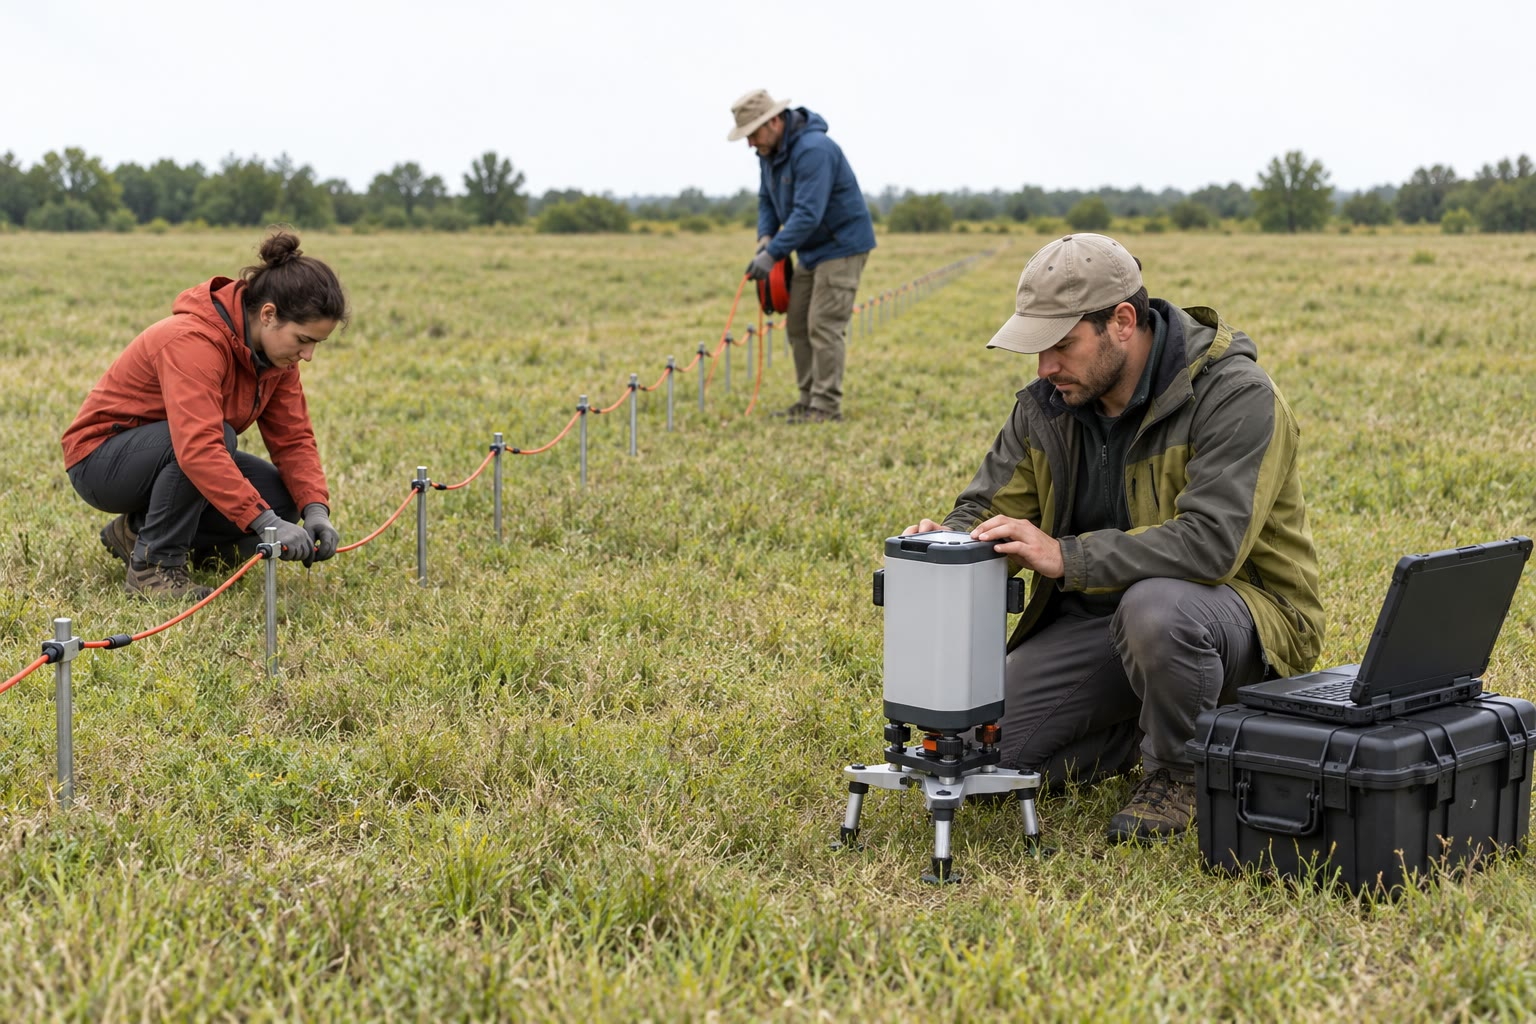
\includegraphics[width=\linewidth]{images/book5/ai/b3-geophysics-crew.jpg}

{\scriptsize 一支地球物理测量组正在铺设电阻率电缆，
其底座上放着一台重力仪（AI 生成插图）。}
\end{minipage}
\end{inthefield}

\begin{example}[瓦尔登测量]\label{ex:b3:field-lab-methods-3:varden}
重力图显示一个闭合低值，约为 \qty{-2.3}{\milli\gal}，
以花岗岩为中心，沿南–北方向拉长：密度较小的花岗岩
向覆盖层之下延伸，且在该方向上最长。低值
从露头向外延伸约 \qty{1}{km}，因此岩体随深度增大而变宽。
其半宽给出等价球体的第一个深度估计；
带竖直侧面与底面的模型表明，底面深度介于一
至几千米之间时，同样能很好地解释峰值，误差在零点几毫伽以内，
因此底面深度仍未知，即上一节所述的非唯一性。
花岗岩上方的谷底，测深曲线起始于干燥砾石的电阻率，
在电流进入饱和水的冲积层处下降，随后
沿斜率为一的直线上升：这是覆盖在高电阻基底上的导电覆盖层，
基底为几米深处的花岗岩。
沿同一谷底拖行的雷达显示出一个平坦回波，约为 \qty{20}{ns}，即地下水位。
此外，磁测线横穿褶皱西翼，此处覆盖层很厚，
基底片岩位于地下约两百米，
记录到一个对称高值，约为 \qty{20}{nT}，任何图件都无法解释：一条镁铁质岩墙，
富含磁铁矿，埋藏于覆盖层之下；
其走向沿磁子午线，这正是异常呈对称的原因。
地球物理学家将其报告为一条辉绿岩岩墙，于不整合面处被截断，
而图上的覆盖层将其掩盖。
周末问题要处理的是
本次测量的数据。
\end{example}
% ledger: gpg:susceptibility, gpg:resistivity, gpg:gpr-table

\section{练习}

\begin{exercise}[$\star$]\label{exo:b3:field-lab-methods-3:1}
(a)~$g = \qty{9.81}{m.s^{-2}}$ 的几分之几是 \qty{0.01}{\milli\gal}？
(b)~重力仪须升高多少，读数才会
仅因自由空气效应改变 \qty{0.01}{\milli\gal}？(c)~同时计入自由空气效应与布格效应，
并取密度为
\qty{2670}{kg.m^{-3}}，结果如何？
\end{exercise}

\begin{exercise}[$\star$]\label{exo:b3:field-lab-methods-3:2}
一个半径为 \qty{50}{m}、密度差为
\qty{+500}{kg.m^{-3}} 的球体，球心位于深 \qty{100}{m} 处。求其
超额质量、异常峰值与半宽 $x_{1/2}$。
\end{exercise}

\begin{exercise}[$\star$]\label{exo:b3:field-lab-methods-3:3}
温纳排列的间距为 $a = \qty{10}{m}$，注入 \qty{0.1}{A} 电流，
测得 \qty{0.239}{V}。(a)~计算几何因子与
\omterm{def:b3:field-lab-methods-3:resistivity}{视电阻率}。(b)~证明取 $s =
\qty{15}{m}$、$l = \qty{5}{m}$ 的施伦贝格尔排列
具有相同的几何因子，并说明原因。
\end{exercise}

\begin{exercise}[$\star$]\label{exo:b3:field-lab-methods-3:4}
花岗岩的 $\varepsilon_r = 5$。(a)~计算雷达波速。(b)~
断口位于地下 \qty{10}{m}，计算其回波的双程走时。
(c)~取 $\sigma = \qty{1}{mS.m^{-1}}$，计算趋肤深度与
约三倍趋肤深度的有效探测深度。(d)~将其与
$\varepsilon_r = 20$、$\sigma = \qty{10}{mS.m^{-1}}$ 的湿黏土比较。
\end{exercise}

\begin{exercise}[$\star\star$]\label{exo:b3:field-lab-methods-3:5}
(a)~推导半径为 $R$、
密度差为 $\Delta\rho$、轴线位于深度 $z$ 处的长水平圆柱体的异常，
由线质量的异常出发推导，并证明 $z = x_{1/2}$。(b)~一个圆柱体与一个球体
峰值相同，半宽同为 $x_{1/2} = \qty{100}{m}$，
比较它们的深度，哪种解释给出更深的岩体？
\end{exercise}

\begin{exercise}[$\star\star$]\label{exo:b3:field-lab-methods-3:6}
瓦尔登花岗岩模型的布格异常，每隔
\qty{100}{m} 取样，图上共 \num{1120} 个点，覆盖范围为 $\qty{3.5}{km}
\times \qty{3.2}{km}$，各点之和为 \qty{-438}{\milli\gal}。(a)~应用
\cref{prop:b3:field-lab-methods-3:gauss} 估算质量亏损。
(b)~模型的质量亏损为 \qty{1.74e11}{kg}。地图恢复了多大比例，
其余部分位于何处？
\end{exercise}

\begin{exercise}[$\star\star$]\label{exo:b3:field-lab-methods-3:7}
(a)~一薄岩墙顶部位于地下 \qty{30}{m}。按“每个半宽取三个读数”的规则，
其中半宽指异常在峰值一半处的全宽，
测点间距应取多少？(b)~对顶部位于地下
\qty{220}{m} 深的情形，同样求解。(c)~为何单次测量
无法同时分辨浅层与深层岩体，除非
它是为浅层岩体而设计的？
\end{exercise}

\begin{exercise}[$\star\star$]\label{exo:b3:field-lab-methods-3:8}
一块被电阻率为 \qty{8}{\ohm\metre} 的水饱和的砂岩，
其电阻率为 \qty{80}{\ohm\metre}。(a)~取 $a = 1$、$m = 2$，
求其孔隙度。(b)~取 $m = 1.8$ 与 $m = 2.2$ 重复计算。测量中的哪一
项决定了孔隙度的不确定度？
\end{exercise}

\begin{exercise}[$\star\star$]\label{exo:b3:field-lab-methods-3:9}
(a)~求两层级数的前三项，
\cref{prop:b3:field-lab-methods-3:layers}在 $s = 2h_1$ 处，取 $k =
\num{0.5}$ 与 $k = \num{-0.5}$ 两种情形，并求它们给出的
\omterm{def:b3:field-lab-methods-3:resistivity}{视电阻率}。(b)~求 $\rho_a/\rho_1$ 在 $s \ll h_1$ 与
$s \gg h_1$ 时的极限；(c)~电阻率比 $\rho_2/\rho_1$ 为何值时对应于
$k = \pm 0.5$？
\end{exercise}

\begin{exercise}[$\star\star\star$]\label{exo:b3:field-lab-methods-3:10}
(a)~求温纳排列的几何因子，需从
\cref{thm:b3:field-lab-methods-3:point-source}出发推导。(b)~求施伦贝格尔排列的
几何因子，并证明 $\rho_a \to 2\pi s^2(-\mathrm{d}V/
\mathrm{d}r)/I$ 在 $l/s \to 0$ 时成立。(c)~近似因子
$\pi s^2/(2l)$ 比精确值高估了多少，当 $l = s/10$ 时？
\end{exercise}

\begin{exercise}[$\star\star\star$]\label{exo:b3:field-lab-methods-3:11}
测站位于基点以上 \qty{50}{m} 处，其读数精度为
\qty{0.01}{\milli\gal}，高度精确到 \qty{5}{cm}；板片密度的
不确定度为 \qty{100}{kg.m^{-3}}，\omterm{def:b3:field-lab-methods-3:terrain}{地形校正}的
不确定度为 \qty{0.2}{\milli\gal}。(a)~列出其布格
异常的误差预算。(b)~哪一项起主导作用，要探测
\qty{0.1}{\milli\gal} 的异常应改进哪一项？(c)~不计
地形项时的总误差为多少？
\end{exercise}

\begin{exercise}[$\star\star\star$]\label{exo:b3:field-lab-methods-3:12}
沿一埋藏体测得五个重力读数，位置为 $x = -600$、$-300$、$0$、
$300$ 与 \qty{600}{m} 处，读数分别为 \num{-0.69}、\num{-2.17}、\num{-4.16}、
\num{-2.10} 与 \qty{-0.73}{\milli\gal}，每个读数的 $\sigma =
\qty{0.03}{\milli\gal}$。(a)~对球心位于 $x = 0$ 正下方、
深度分别为 \num{300}、\num{400} 与 \qty{500}{m} 的球体模型，取使中心读数拟合的质量，
并计算各模型的\omterm{def:b3:field-lab-methods-3:inversion-practice}{拟合差} $\chi^2$。(b)~哪一个
模型在误差范围内与数据相符？(c)~另一形状的
物体能否同样拟合？由什么来判定？
\end{exercise}

\section{问题：瓦尔登丘陵中的隐伏体}

\begin{problem}[{周末问题——整理瓦尔登测量数据}]
\label{pb:b3:field-lab-methods-3:1}
取 $G = \qty{6.674e-11}{m^3.kg^{-1}.s^{-2}}$，自由空气梯度
\qty{0.3086}{\milli\gal.m^{-1}}，布格系数为
\qty{0.1119}{\milli\gal.m^{-1}}（密度 \qty{2670}{kg.m^{-3}}）。

\medskip\noindent\textbf{第一部分——重力闭合环线。}重力剖面上的一条闭合环线
给出（读数为校准后的毫伽值，高度为
米，时间为 09:00 起算的小时数）：
\begin{center}
\small
\begin{tabular}{lccccc}
\hline
测站 & 基点 & \qty{3.0}{km} & \qty{3.5}{km} & \qty{4.0}{km} & 基点 \\
\hline
时间 & 0 & 0.5 & 0.9 & 1.3 & 2.0 \\
高度 & 176.1 & 149.0 & 145.5 & 158.0 & 176.1 \\
读数 & 2846.512 & 2851.075 & 2850.497 & 2849.392 & 2846.708 \\
\hline
\end{tabular}
\end{center}
\begin{enumerate}
\item 求该闭合环线的漂移速率。
\item 对三个测站读数作漂移校正，
  相对于基点表示。
\item 对高度差作自由空气校正与布格校正，
  并求出各测站相对于
  基点的布格异常。
\item 仅仪器本身的漂移为 \qty{0.040}{\milli\gal.h^{-1}}，
  基点处的其余变化由何引起？为何可以
  随漂移一并扣除？
\item 读数所对应的模型给出三个相对于基点的
  异常值，分别为 \num{-0.825}、\num{-2.131} 与
  \qty{-0.825}{\milli\gal}。求整理结果的误差。表中的
  高度已四舍五入至 \qty{0.1}{m}，这会引入怎样的误差，
  这一舍入能否解释这些误差？
\item 要使整理后的异常保持在
  \qty{0.01}{\milli\gal} 以内，需要多高的高度精度？测量手册
  为何要求 \qty{3.3}{cm} 这样更严格的数值？
\end{enumerate}

\medskip\noindent\textbf{第二部分——花岗岩的异常。}沿剖面，异常
的极小值为 \qty{-2.293}{\milli\gal}，位于
$x = \qty{3.50}{km}$ 处，并在 $x = 3.048$ 与
\qty{3.952}{km} 处取得该值的一半。花岗岩模型的密度差为
\qty{-130}{kg.m^{-3}}，中心处的地面高出
海平面 \qty{145.5}{m}。
\begin{enumerate}[resume]
\item 求半宽 $x_{1/2}$ 及等效球体中心的
  深度。
\item 求该球体的质量亏损，以及在花岗岩密度差下的
  半径。结果有何异常之处？
\item 该模型的质心位于地面以下 \qty{864}{m}，其
  质量亏损为 \qty{1.74e11}{kg}。为何半宽法给出的
  是更浅、更轻的物体？
\item 一个竖直圆柱体，其面积与花岗岩在不整合处的
  面积相同，半径为 \qty{461}{m}。求其轴线上的异常，
  取顶面位于地面、底面位于 \qty{1645}{m} 深处的情形，以及
  深度无限大的情形。
\item 用试算或求解的方法，求出使该圆柱体
  给出观测值 \qty{-2.29}{\milli\gal} 的底面深度。
\item 求顶面位于地下 \qty{6}{m} 时该圆柱体的异常
  （底面 \qty{1645}{m}）。重力能否判断花岗岩
  是否在冲积层之下一直延伸至地表？
\end{enumerate}

\medskip\noindent\textbf{第三部分——谷底。}花岗岩上方谷底的施伦贝格尔
电测深给出（半间距 $s$ 的单位为
米，$\rho_a$ 的单位为 \unit{\ohm\metre}）：
\begin{center}
\small
\begin{tabular}{lcccccccc}
\hline
$s$ & 1 & 2 & 4 & 6 & 10 & 20 & 30 & 40 \\
$\rho_a$ & 577 & 526 & 387 & 350 & 449 & 821 & 1309 & 1684 \\
\hline
\end{tabular}
\end{center}
沿同一谷底的雷达剖面上，一条管线给出一条双曲线，
其顶点处为 \qty{10.7}{ns}，在旁侧 \qty{1}{m} 处的走时
为 \qty{17.1}{ns}；平直回波在 \qty{20.0}{ns} 到达。
\begin{enumerate}[resume]
\item 当 $s = \qty{20}{m}$ 时，MN 长 \qty{2}{m}，电流为
  \qty{50}{mA}。求几何因子及所测电压。
\item 求雷达波速、冲积层的相对介电常数，以及
  管线的深度。
\item 平直回波对应地下水位，其深度为多少？
\item 利用
  20、30 与 \qty{40}{m} 处的读数，估算冲积层的电导 $S$。
\item 干燥冲积层的电阻率为 \qty{600}{\ohm\metre}，饱和
  冲积层为 \qty{222}{\ohm\metre}。求饱和冲积层的厚度，以及
  花岗岩顶面的深度。该估计偏高还是偏低，
  原因何在？
\item 地下水的电阻率为 \qty{20}{\ohm\metre}。求
  冲积层的孔隙度，用\omterm{prop:b3:field-lab-methods-3:archie}{阿奇定律}，取 $m = 2$，并求 $m$
  介于 \num{1.3} 与 \num{2.8} 之间时的取值范围。
\end{enumerate}

\medskip\noindent\textbf{第四部分——磁力线。}测线
自 $x = \qty{1.70}{km}$ 处向东延伸，每隔 \qty{50}{m} 设一个测点，
每两分钟测量一次；基站在相同的分钟记录数据。
各读数减去 \qty{48000}{nT} 后为：
\begin{center}
\small
\setlength{\tabcolsep}{3.5pt}
\begin{tabular}{lccccccccccc}
\hline
$x$（千米） & 1.70 & 1.75 & 1.80 & 1.85 & 1.90 & 1.95 & 2.00 & 2.05 & 2.10 & 2.15 & 2.20 \\
线路 & 3.4 & 4.8 & 6.3 & 8.1 & 10.3 & 12.8 & 15.8 & 19.2 & 22.9 & 26.2 & 28.0 \\
基站 & 0.0 & 0.7 & 1.5 & 2.2 & 2.9 & 3.6 & 4.3 & 5.0 & 5.7 & 6.4 & 7.0 \\
\hline
$x$（千米） & 2.25 & 2.30 & 2.35 & 2.40 & 2.45 & 2.50 & 2.55 & 2.60 & 2.65 & 2.70 & \\
线路 & 27.7 & 25.8 & 23.3 & 20.9 & 19.0 & 17.6 & 16.6 & 15.9 & 15.5 & 15.2 & \\
基站 & 7.6 & 8.2 & 8.8 & 9.4 & 9.9 & 10.4 & 10.9 & 11.3 & 11.7 & 12.1 & \\
\hline
\end{tabular}
\end{center}
主磁场为 \qty{48000}{nT}，倾角为 \ang{65}。
\begin{enumerate}[resume]
\item 进行\omterm{def:b3:field-lab-methods-3:magnetic}{日变校正}，并给出
  各测点校正后的异常值。
\item 证明：若不作校正，东侧异常值
  永远不会降至其峰值的一半。
\item 确定峰值位置，以及校正后异常值等于峰值一半的两点，
  用线性插值法求得，并计算半宽。
\item 该异常是对称的。这说明了该体的走向
  有何特点？半宽法则假设的是哪一类体？
\item 计算磁化率与厚度的乘积 $\kappa t$。
  若岩墙为磁化率为 \num{0.03} 的辉绿岩，
  则其厚度为多少？
\item 测点间距是否足够小？
\item 求隐伏岩墙顶面在地表以下的深度（精确到十米），
  并与该地区地质模型中此处的
  不整合面深度作比较，该深度为
  \qty{222}{m}。
\end{enumerate}
\end{problem}
% ledger: gpg:grav-survey, gpg:mag-field, keys:archie
